\documentclass{book}

% load packages
\usepackage{geometry}
\usepackage{hyperref,bookmark}
\usepackage{xcolor}
\usepackage{graphicx}
\usepackage{etoolbox}

%% Set page size
\geometry{a4paper, total={170mm,257mm}, left=25mm, top=20mm, bottom=20mm, right=25mm}

%% Set colours
\definecolor{light}{HTML}{E6E6FA}
\definecolor{highlight}{HTML}{800080}
\definecolor{dark}{HTML}{330033}

% We will generate all images so they have a width \maxwidth. This means
% that they will get their normal width if they fit onto the page, but
% are scaled down if they would overflow the margins.
\makeatletter
\def\maxwidth{\ifdim\Gin@nat@width>\linewidth\linewidth
\else\Gin@nat@width\fi}
\makeatother
\let\Oldincludegraphics\includegraphics
\renewcommand{\includegraphics}[1]{\Oldincludegraphics[width=\maxwidth]{#1}}


\begin{document}

\title{Die barocken Schloss- und Gartenveduten}
\usepackage{etoolbox}
\makeatletter
\providecommand{\subtitle}[1]{% add subtitle to \maketitle
  \apptocmd{\@title}{\par {\large #1 \par}}{}{}
}
\makeatother
\subtitle{Ein Versuch eines PDF-Buchs}
\author{AR}
\date{2024-06-15}
 

\frontmatter
\maketitle

\renewcommand*\contentsname{Table of contents}
{
\setcounter{tocdepth}{2}
\tableofcontents
}

\bookmarksetup{startatroot}

\chapter{Katalog zur Ausstellung: Die barocken Schloss- und
Gartenveduten}\label{katalog-zur-ausstellung-die-barocken-schloss--und-gartenveduten}

Ein Katalog mit Kunstwerken aus der CbDD-Sammlung. Textteil:
\href{https://www.deckenmalerei.eu/42d06165-58e7-4653-bfe4-3d5f7091fc33\#6e73f774-4b7f-4e37-937b-e11cc35c5bc8}{6e73f774-4b7f-4e37-937b-e11cc35c5bc8}

Die barocken Schloss- und Gartenveduten {[}Sammlung{]}

This work is licensed under a Creative Commons
Attribution-NonCommercial-NoDerivs 4.0 International License.

\bookmarksetup{startatroot}

\chapter{Die barocken Schloss- und
Gartenveduten}\label{die-barocken-schloss--und-gartenveduten}

Wikibase link:
\url{https://computational-publishing-service.wikibase.cloud/entity/Q282}

Kurator: Seeger, Ulrike

\paragraph{Die barocken Schloss- und
Gartenveduten}\label{die-barocken-schloss--und-gartenveduten-1}

\subparagraph{Entstehungs- und
Erhaltungsgeschichte}\label{entstehungs--und-erhaltungsgeschichte}

Eine weitere Bereicherung erfuhr die Saalausstattung des Barock im
Rechnungsjahr 1715/16 durch die ringsumlaufenden Lambris von Christian
Thalwitzer.{[}1{]} 51 längsrechteckige Felder wurden mit Gemälden nach
zeitgenössischen Schloss- und Gartenveduten versehen. In den
Fensterlaibungen nahmen 27 hochrechteckige Felder Abbildungen von
Orangenbäumen und anderen exotischen Kübelpflanzen auf. Die Ansicht des
Carlsbergs bei Weikersheim, die erst 1747 im Zusammenhang mit der damals
aufgestellten Kunstuhr hinzukam, dürfte eine ältere Vedute ersetzt
haben, die sich am Fensterpfeiler hinter der Uhr noch befinden könnte.

\textbf{Beschreibung und Ikonographie}

Die Veduten, deren Vorlagen durchgehend zu benennen sind, wurden am
oberen Rahmen mit einem Spruchband beschriftet. Sie lassen sich also
leicht zuordnen.{[}2{]} Indem die erläuternden Beischriften direkt von
den graphischen Vorlagen übernommen wurden, führten sie die Tradition
der Deckengemälde Balthasar Katzenbergers aus der Renaissance weiter.
Der Schwerpunkt der Veduten lag auf Frankreich, von wo 30 Ansichten
vornehmlich nach Pérelle übernommen wurden. Außer Gebäuden und Gärten in
Paris und Versailles waren die Landschlösser Richelieu, Liancourt,
St.~Cloud, St.-Germain-en-Laye, Chantilly, Clagny und Vaux-le-Vicomte
vertreten sowie von Paris die Stadttore Porte St.~Antoine, Porte
St.~Denis und Arc de triomphe. Die Ansicht des Marktplatzes von Naxos
gehörte insofern zu den französischen Veduten, als sie das in Paris von
Aveline gestochene Bühnenbild Giacomo Torellis einer in Venedig
aufgeführten Oper wiedergab.{[}3{]}

Lediglich sechs Veduten bezogen sich auf reichsfürstliche Anlagen.
Salzdahlum des Herzogs Anton Ulrich von Braunschweig-Wolfenbüttel war
mit Hof- und Gartenseite zu sehen. Schloss Philippsruhe bei
Hanau-Kesselstadt am Main wurde nach der 1705 erschienenen Ansicht
abgebildet.{[}4{]}Drei Vogelschauen von Schloss Ludwigsburg Herzog
Eberhard Ludwigs von Württemberg entstammen dem 1711 erschienenen
Stichwerk von Johann Friedrich Nette.{[}5{]} Hinzu kamen eine Ansicht
von Weikersheim mit Lustgarten und des nahegelegenen Lustgartens in
Schäftersheim. Beide Anlagen lagen nicht als Stiche vor, wurden aber
dennoch in dieser Art abgebildet. Holländische Stiche wurden in den
Zyklus nicht einbezogen.

Thalwitzer steigerte die Lesbarkeit der Veduten, indem er sie in Farbe
malte und in ihrem Formenreichtum vereinfachte. Außerdem reduzierte er
das bei Pérelle und seinen Nachfolgern stets große Aufgebot an
Staffagefiguren. Größeren Wert als Pérelle legte er hingegen auf
Stadtsilhouetten oder auch Berge im Hintergrund. Vereinheitlichend
wirkte sein gleichmäßiges Himmelsblau mit waagrecht bildparallel
dahinziehenden Wolken. Es fand sich in der gleichen Art, jedoch über
tiefliegendem Horizont auf den Veduten der exotischen Kübelgewächse.

\textbf{Anordnung}

Eine gewisse Ordnung lässt sich lediglich an der Westwand erkennen, wo
die Veduten zu beiden Seiten des Kamins symmetrisch beginnen. Flankiert
wird der Kamin von zwei Gartenansichten von Versailles, an die sich je
eine Ansicht von Paris und als erste Vedute der Längsseite die Ansicht
eines Landschlosses (Salzdahlum und Liancourt) anschließen. Ansonsten
regiert das Prinzip der Vielfalt, indem beispielsweise die Serie der
Pariser Stadttore über die gesamten Lambris verteilt ist.

\subparagraph{\texorpdfstring{\textbf{Erhaltungszustand}}{Erhaltungszustand}}\label{erhaltungszustand}

Wie alle Lambrisgemälde Christian Thalwitzers wurden auch die Schloss-
und Gartenveduten des Rittersaals nach 1945 von Prinz Constantin
restaurierend übermalt.{[}6{]}

{[}1{]} Die Datierung verdankt die Autorin einer Mitteilung von Dinah
Rottschäfer.

{[}2{]} Die Sujets aufgeführt bei Merten, Weikersheim, o. J., S. 45--46.
Eine der als „ungeklärt`` bezeichneten Veduten stellt Schloss Richelieu
dar.

{[}3{]} Die Legende des Stichs von Aveline nach Torelli lautet: „ La
Grande place de la Ville de Naxos, qui est une decoration du second Acte
de l'Opera de VENUS IALOUSE {[}= Venere Gelosa{]} representé à Venise.
Inventé par Jacques Torellj de Fano en Italie et Gravé par Aveline a
Paris ».

{[}4{]} https://www.lagis-hessen.de/de/subjects/idrec/sn/oa/id/1708
„Ansicht von Schloss Philippsruhe, 1705``, in: Historische Ortsansichten
\url{https://www.lagis-hessen.de/de/subjects/idrec/sn/oa/id/1708}
(Stand: 23.1.2017)

{[}5{]}
http://digital.wlb-stuttgart.de/sammlungen/sammlungsliste/werksansicht/?no\_cache=1\&tx\_dlf\%5Bid\%5D=2885\&tx\_dlf\%5Bpage\%5D=1

{[}6{]} Wiese, Fürstensitz, 2019, S. 424.

Wikibase link:
\url{https://computational-publishing-service.wikibase.cloud/entity/Q283}

Title: Die barocken Schloss- und Gartenveduten bild

Year: 2018

Description: Bild für Die barocken Schloss- und Gartenveduten

Wikibase link:
\url{https://computational-publishing-service.wikibase.cloud/entity/Q283}

Title: Die barocken Schloss- und Gartenveduten bild

Year: 2018-01-01T00:00:00Z

Description: Bild für Die barocken Schloss- und Gartenveduten

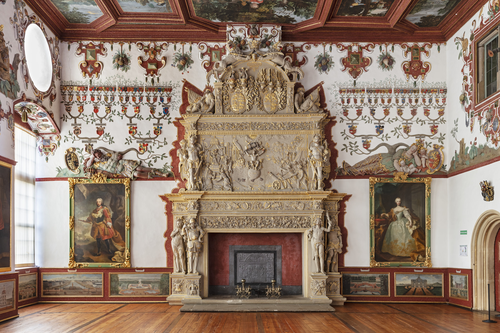
\includegraphics{section_files/figure-pdf/cell-4-output-2.png}
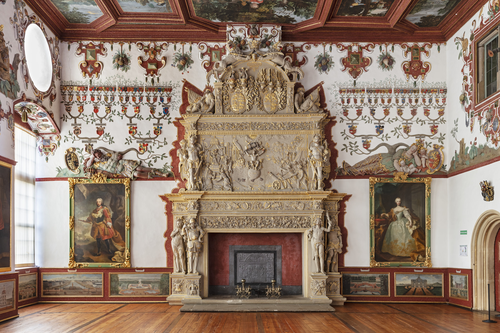
\includegraphics{section_files/figure-pdf/cell-4-output-3.png}

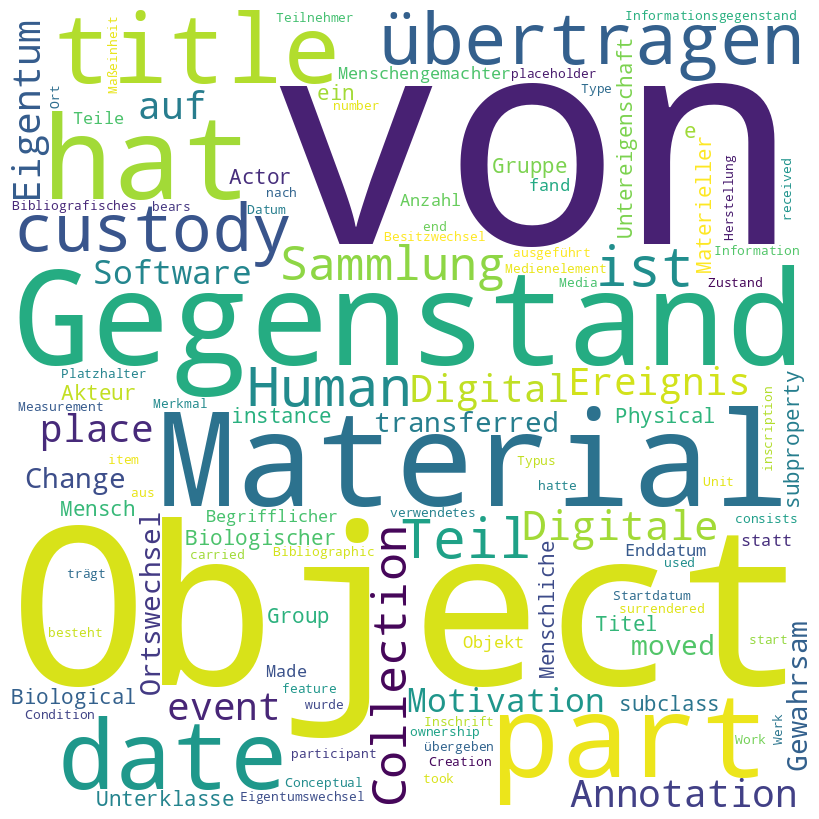
\includegraphics{section_files/figure-pdf/cell-5-output-1.png}

\end{document}
